\begin{flushright}
    در ادامه با شناسایی الگوهای تکراری مانند حلقه و یا تابع در زبان اسمبلی، سطح انتزاع فراتری که زبان‌های سطح بالا شناخته می‌شوند، ایجاد شد.
    تصویر زیر یک مثال از \textbf{پیاده‌سازی} حلقه در اسمبلی و \textbf{انتزاع} آن در زبان سطح بالاتر می‌باشد.

    \begin{figure}[H]
        \centering
        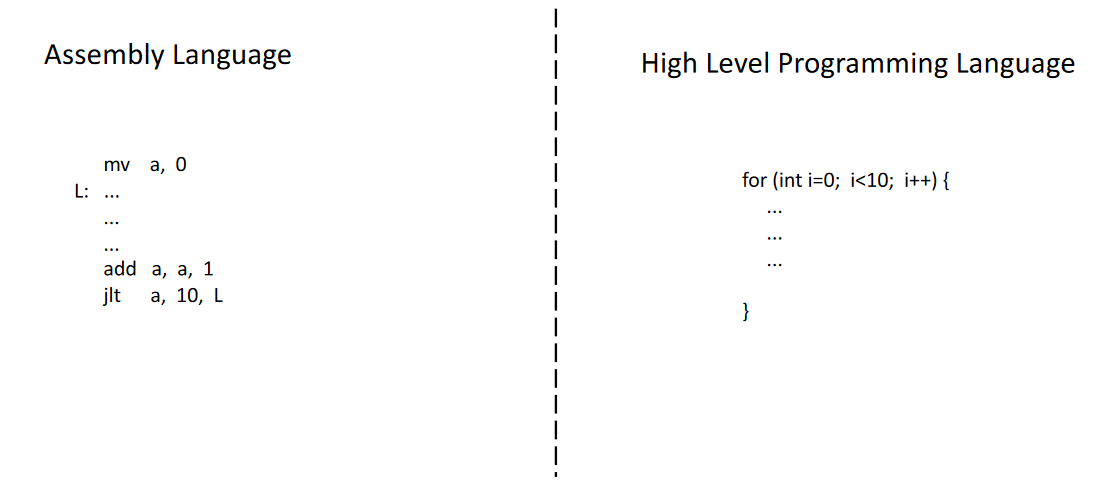
\includegraphics[width=0.8\textwidth]{source/high-level-programming-language-imp&abs}
        \caption{پیاده‌سازی حلقه در زبان اسمبلی}
        \label{fig:for-in-assembly}
    \end{figure}
\end{flushright}